\documentclass[25pt, a0paper, portrait, margin=0mm, innermargin=15mm,
blockverticalspace=10mm, colspace=15mm, subcolspace=8mm]{tikzposter}

\usepackage{times}
\usepackage{microtype}
\usepackage{booktabs}
\usepackage{mathptmx}
\usepackage{graphicx}
\usepackage{url}
\usepackage{listings}
\usepackage{hyperref}
\usepackage{underscore}
\usepackage[T1]{fontenc}
\usepackage{amsmath}
\usepackage{amsfonts}
\usepackage{amssymb}
\usepackage{verbatim}
\usepackage{color}
\usepackage{xspace}
\usepackage{multirow}
\usepackage{relsize}
\usepackage{fancyvrb}
\usepackage{pgfplots}
\usepackage{adjustbox}
\title{Nail: A practical tool for parsing and generating data formats}
\author{Julian Bangert and Nickolai Zeldovich }
\institute{MIT CSAIL}
%\titlegraphic{Logo}
\usetheme{Envelope}


\makeatletter
\def\PY@reset{\let\PY@it=\relax \let\PY@bf=\relax%
    \let\PY@ul=\relax \let\PY@tc=\relax%
    \let\PY@bc=\relax \let\PY@ff=\relax}
\def\PY@tok#1{\csname PY@tok@#1\endcsname}
\def\PY@toks#1+{\ifx\relax#1\empty\else%
    \PY@tok{#1}\expandafter\PY@toks\fi}
\def\PY@do#1{\PY@bc{\PY@tc{\PY@ul{%
    \PY@it{\PY@bf{\PY@ff{#1}}}}}}}
\def\PY#1#2{\PY@reset\PY@toks#1+\relax+\PY@do{#2}}

\expandafter\def\csname PY@tok@gd\endcsname{\def\PY@tc##1{\textcolor[rgb]{0.63,0.00,0.00}{##1}}}
\expandafter\def\csname PY@tok@gu\endcsname{\let\PY@bf=\textbf\def\PY@tc##1{\textcolor[rgb]{0.50,0.00,0.50}{##1}}}
\expandafter\def\csname PY@tok@gt\endcsname{\def\PY@tc##1{\textcolor[rgb]{0.00,0.27,0.87}{##1}}}
\expandafter\def\csname PY@tok@gs\endcsname{\let\PY@bf=\textbf}
\expandafter\def\csname PY@tok@gr\endcsname{\def\PY@tc##1{\textcolor[rgb]{1.00,0.00,0.00}{##1}}}
\expandafter\def\csname PY@tok@cm\endcsname{\let\PY@it=\textit\def\PY@tc##1{\textcolor[rgb]{0.25,0.50,0.50}{##1}}}
\expandafter\def\csname PY@tok@vg\endcsname{\def\PY@tc##1{\textcolor[rgb]{0.10,0.09,0.49}{##1}}}
\expandafter\def\csname PY@tok@mh\endcsname{\def\PY@tc##1{\textcolor[rgb]{0.40,0.40,0.40}{##1}}}
\expandafter\def\csname PY@tok@go\endcsname{\def\PY@tc##1{\textcolor[rgb]{0.53,0.53,0.53}{##1}}}
\expandafter\def\csname PY@tok@ge\endcsname{\let\PY@it=\textit}
\expandafter\def\csname PY@tok@vc\endcsname{\def\PY@tc##1{\textcolor[rgb]{0.10,0.09,0.49}{##1}}}
\expandafter\def\csname PY@tok@il\endcsname{\def\PY@tc##1{\textcolor[rgb]{0.40,0.40,0.40}{##1}}}
\expandafter\def\csname PY@tok@cs\endcsname{\let\PY@it=\textit\def\PY@tc##1{\textcolor[rgb]{0.25,0.50,0.50}{##1}}}
\expandafter\def\csname PY@tok@cp\endcsname{\def\PY@tc##1{\textcolor[rgb]{0.74,0.48,0.00}{##1}}}
\expandafter\def\csname PY@tok@gi\endcsname{\def\PY@tc##1{\textcolor[rgb]{0.00,0.63,0.00}{##1}}}
\expandafter\def\csname PY@tok@gh\endcsname{\let\PY@bf=\textbf\def\PY@tc##1{\textcolor[rgb]{0.00,0.00,0.50}{##1}}}
\expandafter\def\csname PY@tok@ni\endcsname{\let\PY@bf=\textbf\def\PY@tc##1{\textcolor[rgb]{0.60,0.60,0.60}{##1}}}
\expandafter\def\csname PY@tok@nl\endcsname{\def\PY@tc##1{\textcolor[rgb]{0.63,0.63,0.00}{##1}}}
\expandafter\def\csname PY@tok@nn\endcsname{\let\PY@bf=\textbf\def\PY@tc##1{\textcolor[rgb]{0.00,0.00,1.00}{##1}}}
\expandafter\def\csname PY@tok@no\endcsname{\def\PY@tc##1{\textcolor[rgb]{0.53,0.00,0.00}{##1}}}
\expandafter\def\csname PY@tok@na\endcsname{\def\PY@tc##1{\textcolor[rgb]{0.49,0.56,0.16}{##1}}}
\expandafter\def\csname PY@tok@nb\endcsname{\def\PY@tc##1{\textcolor[rgb]{0.00,0.50,0.00}{##1}}}
\expandafter\def\csname PY@tok@nc\endcsname{\let\PY@bf=\textbf\def\PY@tc##1{\textcolor[rgb]{0.00,0.00,1.00}{##1}}}
\expandafter\def\csname PY@tok@nd\endcsname{\def\PY@tc##1{\textcolor[rgb]{0.67,0.13,1.00}{##1}}}
\expandafter\def\csname PY@tok@ne\endcsname{\let\PY@bf=\textbf\def\PY@tc##1{\textcolor[rgb]{0.82,0.25,0.23}{##1}}}
\expandafter\def\csname PY@tok@nf\endcsname{\def\PY@tc##1{\textcolor[rgb]{0.00,0.00,1.00}{##1}}}
\expandafter\def\csname PY@tok@si\endcsname{\let\PY@bf=\textbf\def\PY@tc##1{\textcolor[rgb]{0.73,0.40,0.53}{##1}}}
\expandafter\def\csname PY@tok@s2\endcsname{\def\PY@tc##1{\textcolor[rgb]{0.73,0.13,0.13}{##1}}}
\expandafter\def\csname PY@tok@vi\endcsname{\def\PY@tc##1{\textcolor[rgb]{0.10,0.09,0.49}{##1}}}
\expandafter\def\csname PY@tok@nt\endcsname{\let\PY@bf=\textbf\def\PY@tc##1{\textcolor[rgb]{0.00,0.50,0.00}{##1}}}
\expandafter\def\csname PY@tok@nv\endcsname{\def\PY@tc##1{\textcolor[rgb]{0.10,0.09,0.49}{##1}}}
\expandafter\def\csname PY@tok@s1\endcsname{\def\PY@tc##1{\textcolor[rgb]{0.73,0.13,0.13}{##1}}}
\expandafter\def\csname PY@tok@sh\endcsname{\def\PY@tc##1{\textcolor[rgb]{0.73,0.13,0.13}{##1}}}
\expandafter\def\csname PY@tok@sc\endcsname{\def\PY@tc##1{\textcolor[rgb]{0.73,0.13,0.13}{##1}}}
\expandafter\def\csname PY@tok@sx\endcsname{\def\PY@tc##1{\textcolor[rgb]{0.00,0.50,0.00}{##1}}}
\expandafter\def\csname PY@tok@bp\endcsname{\def\PY@tc##1{\textcolor[rgb]{0.00,0.50,0.00}{##1}}}
\expandafter\def\csname PY@tok@c1\endcsname{\let\PY@it=\textit\def\PY@tc##1{\textcolor[rgb]{0.25,0.50,0.50}{##1}}}
\expandafter\def\csname PY@tok@kc\endcsname{\let\PY@bf=\textbf\def\PY@tc##1{\textcolor[rgb]{0.00,0.50,0.00}{##1}}}
\expandafter\def\csname PY@tok@c\endcsname{\let\PY@it=\textit\def\PY@tc##1{\textcolor[rgb]{0.25,0.50,0.50}{##1}}}
\expandafter\def\csname PY@tok@mf\endcsname{\def\PY@tc##1{\textcolor[rgb]{0.40,0.40,0.40}{##1}}}
%\expandafter\def\csname PY@tok@err\endcsname{\def\PY@bc##1{\setlength{\fboxsep}{0pt}\fcolorbox[rgb]{1.00,0.00,0.00}{1,1,1}{\strut ##1}}}
\expandafter\def\csname PY@tok@kd\endcsname{\let\PY@bf=\textbf\def\PY@tc##1{\textcolor[rgb]{0.00,0.50,0.00}{##1}}}
\expandafter\def\csname PY@tok@ss\endcsname{\def\PY@tc##1{\textcolor[rgb]{0.10,0.09,0.49}{##1}}}
\expandafter\def\csname PY@tok@sr\endcsname{\def\PY@tc##1{\textcolor[rgb]{0.73,0.40,0.53}{##1}}}
\expandafter\def\csname PY@tok@mo\endcsname{\def\PY@tc##1{\textcolor[rgb]{0.40,0.40,0.40}{##1}}}
\expandafter\def\csname PY@tok@kn\endcsname{\let\PY@bf=\textbf\def\PY@tc##1{\textcolor[rgb]{0.00,0.50,0.00}{##1}}}
\expandafter\def\csname PY@tok@gp\endcsname{\let\PY@bf=\textbf\def\PY@tc##1{\textcolor[rgb]{0.00,0.00,0.50}{##1}}}
\expandafter\def\csname PY@tok@kr\endcsname{\let\PY@bf=\textbf\def\PY@tc##1{\textcolor[rgb]{0.00,0.50,0.00}{##1}}}
\expandafter\def\csname PY@tok@s\endcsname{\def\PY@tc##1{\textcolor[rgb]{0.73,0.13,0.13}{##1}}}
\expandafter\def\csname PY@tok@kp\endcsname{\def\PY@tc##1{\textcolor[rgb]{0.00,0.50,0.00}{##1}}}
\expandafter\def\csname PY@tok@w\endcsname{\def\PY@tc##1{\textcolor[rgb]{0.73,0.73,0.73}{##1}}}
\expandafter\def\csname PY@tok@kt\endcsname{\def\PY@tc##1{\textcolor[rgb]{0.69,0.00,0.25}{##1}}}
\expandafter\def\csname PY@tok@ow\endcsname{\let\PY@bf=\textbf\def\PY@tc##1{\textcolor[rgb]{0.67,0.13,1.00}{##1}}}
\expandafter\def\csname PY@tok@sb\endcsname{\def\PY@tc##1{\textcolor[rgb]{0.73,0.13,0.13}{##1}}}
\expandafter\def\csname PY@tok@k\endcsname{\let\PY@bf=\textbf\def\PY@tc##1{\textcolor[rgb]{0.00,0.50,0.00}{##1}}}
\expandafter\def\csname PY@tok@se\endcsname{\let\PY@bf=\textbf\def\PY@tc##1{\textcolor[rgb]{0.73,0.40,0.13}{##1}}}
\expandafter\def\csname PY@tok@sd\endcsname{\let\PY@it=\textit\def\PY@tc##1{\textcolor[rgb]{0.73,0.13,0.13}{##1}}}

\def\PYZbs{\char`\\}
\def\PYZus{\char`\_}
\def\PYZob{\char`\{}
\def\PYZcb{\char`\}}
\def\PYZca{\char`\^}
\def\PYZam{\char`\&}
\def\PYZlt{\char`\<}
\def\PYZgt{\char`\>}
\def\PYZsh{\char`\#}
\def\PYZpc{\char`\%}
\def\PYZdl{\char`\$}
\def\PYZhy{\char`\-}
\def\PYZsq{\char`\'}
\def\PYZdq{\char`\"}
\def\PYZti{\char`\~}
% for compatibility with earlier versions
\def\PYZat{@}
\def\PYZlb{[}
\def\PYZrb{]}
\makeatother



\begin{document}
\maketitle
\begin{columns}
\column{.5}
\block{Parsing vulnerabilities}{
Current software typically uses hand-implemented parsers, which are not only prone to bugs, but two
separate parser implementations can disagree about the meaning of an input. This has been the source
of many recent high-profile vulnerabilities:
\begin{itemize}
\item Evasi0n jailbreaks on iOS.
\item PKI layer cake.
\item Android master key.
\end{itemize}

{\bf Case study of ZIP vulnerabilities in the CVE database:}

\begin{tabular}{lllr}
\toprule
 \bf Classification  & \bf Example description & \bf Count\\
\midrule
  Memory corruption  & Buffer overflow & 11\\
  Parsing inconsistency & Virus scanners interpret ZIP files incorrectly & 4\\
  Semantic misunderstanding & Weak cryptography used even if user selects AES & 1\\
\midrule
  \multicolumn{2}{l}{\bf Total of all vulnerabilities related to .zip processing }& \bf 16  \\
\bottomrule
  
\end{tabular}
}

\block{State of the art}{   
Grammar-based parsers, such as \texttt{bison} or Hammer, are compact, reuseable
and safer. However, traditional parsers are inconvenient to use, because the programmer has to write all the
yellow-colored parts:

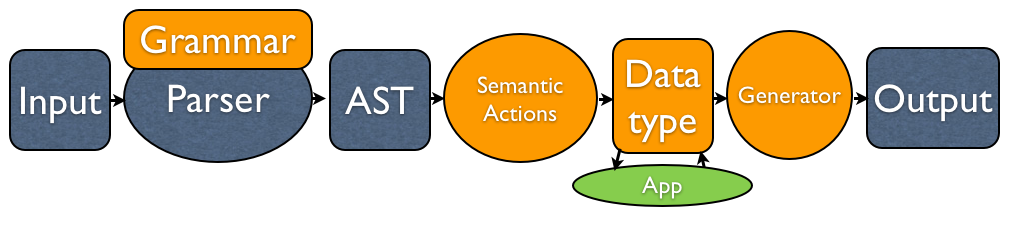
\includegraphics{StateOfTheArt.png}

Nail grammars describe both the format and a data type to represent it, an idea introduced by data
description languages such as PacketTypes. 

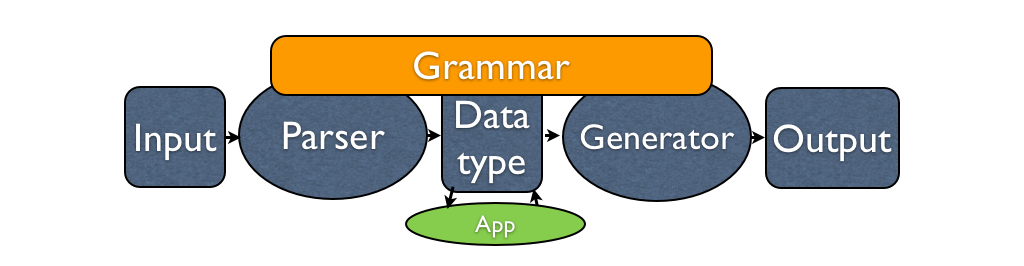
\includegraphics{Nail.png}
  
However, existing solutions cannot handle complicated file formats like ZIP, which feature
duplicated data, offsets and format-specific complications, such as a variable-length end-of-file
header:

\begin{centering}
  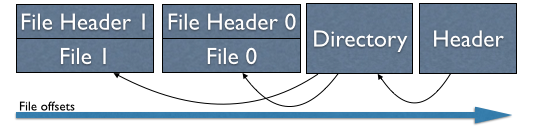
\includegraphics[width=0.35\columnwidth]{ZipHorizontal.png}
\end{centering}
}
\block{Design Goals}{
  \begin{itemize}
    \item Reduce programmer effort
  \begin{itemize}
      \item Semantic combinators describes data type and format.
      \item Generate output. Semantic bijection, preserves meaning, but can change representation.
  \end{itemize}
     \item Handle complex formats
  \begin{itemize}
       \item Dependency Fields: hide redundant and structural information.
       \item Transforms: Extensibility mechanism to capture many features without complicating the
         grammar language.
       \end{itemize}
  \end{itemize}
}
\block{Dependent Fields}{
Duplicated data and layout information can confuse the application, for
example if a length field is not correct or multiple copies of the same data are inconsistent. 
Nail grammars can use Dependent Fields, which are automatically verified during parsing and created during 
generation, to hide such information from the application.
}
\block{Streams and Transformations}{
  Existing parsers are linear, consuming input front to back. Complicated formats require inelegant hacks. 
  Nail grammars feature multiple streams and introduce \emph{Transformations} to create
  them. Transformations are a pair of functions operating on streams and dependent fields.
  A standard library of Transformations is provided, but  programmers can extend
  Nail with custom transformations, which contain arbitrary code and should be carefully written.
%  For example, in the ZIP grammar above, the programmer has to write two functions to find and
%  generate the end-of-file header, with the following prototype:
% \begin{Verbatim}[commandchars=\\\{\},codes={\catcode`\$=3\catcode`\^=7\catcode`\_=8}]
\PY{k+kt}{int}
\PY{n+nf}{dnscompress\PYZus{}parse}\PY{p}{(}\PY{n}{NailArena} \PY{o}{*}\PY{n}{tmp}\PY{p}{,}
                  \PY{n}{NailStream} \PY{o}{*}\PY{n}{out\PYZus{}decomp}\PY{p}{,}
                  \PY{n}{NailStream} \PY{o}{*}\PY{n}{in\PYZus{}current}\PY{p}{)}\PY{p}{;}

\PY{k+kt}{int}
\PY{n+nf}{dnscompress\PYZus{}generate}\PY{p}{(}\PY{n}{NailArena} \PY{o}{*}\PY{n}{tmp}\PY{p}{,}
                     \PY{n}{NailStream} \PY{o}{*}\PY{n}{in\PYZus{}decomp}\PY{p}{,}
                     \PY{n}{NailStream} \PY{o}{*}\PY{n}{out\PYZus{}current}\PY{p}{)}\PY{p}{;}
\end{Verbatim}

}
% \block{Semantic Bijection}{
%   Traditional bijections don't make sense for some data formats. For example, offsets are and should
%   be discarded during parsing. Nail parsers and generators therefore form a looser 'semantic
%   bijection', in which parser(generator(x)) = x, but not necessarily vice versa.

% }
\column{.5}
\block{Nail Grammar for ZIP}{
{\small
\begin{Verbatim}[commandchars=\\\{\},codes={\catcode`\$=3\catcode`\^=7\catcode`\_=8}]
\PY{n}{zip} \PY{o}{=} \PY{p}{\PYZob{}}  \PY{c+cm}{/*cut for brevity*/}
 \PY{err}{\PYZdl{}}\PY{n}{filestream}\PY{p}{,} \PY{err}{\PYZdl{}}\PY{n}{end\PYZus{}directory} \PY{n}{transform} \PY{n}{zip\PYZus{}eod} \PY{p}{(}\PY{err}{\PYZdl{}}\PY{n}{current}\PY{p}{)}
 \PY{n}{contents} \PY{n}{apply} \PY{err}{\PYZdl{}}\PY{n}{end\PYZus{}directory} \PY{n}{end\PYZus{}of\PYZus{}directory}\PY{p}{(}\PY{err}{\PYZdl{}}\PY{n}{filestream}\PY{p}{)}
\PY{p}{\PYZcb{}}
\PY{n}{end\PYZus{}of\PYZus{}directory}\PY{p}{(}\PY{err}{\PYZdl{}}\PY{n}{filestream}\PY{p}{)} \PY{o}{=} \PY{p}{\PYZob{}} 
     \PY{n}{uint32} \PY{o}{=} \PY{l+m+mh}{0x06054b50}
     \PY{n}{disks} \PY{n}{uint16} \PY{o}{|} \PY{p}{[}\PY{l+m+mi}{0}\PY{p}{]}
     \PY{n}{directory\PYZus{}disk} \PY{n}{uint16} \PY{o}{|} \PY{p}{[}\PY{l+m+mi}{0}\PY{p}{]}
     \PY{err}{@}\PY{n}{this\PYZus{}records} \PY{n}{uint16}
     \PY{err}{@}\PY{n}{total\PYZus{}records} \PY{n}{uint16} 
     \PY{n}{transform} \PY{n}{uint16\PYZus{}depend} \PY{p}{(}\PY{err}{@}\PY{n}{this\PYZus{}records} \PY{err}{@}\PY{n}{total\PYZus{}records}\PY{p}{)}
     \PY{err}{@}\PY{n}{directory\PYZus{}size} \PY{n}{uint32} 
     \PY{err}{@}\PY{n}{directory\PYZus{}start} \PY{n}{uint32}
     \PY{err}{\PYZdl{}}\PY{n}{dirstr1} \PY{n}{transform} \PY{n}{offset\PYZus{}u32} \PY{p}{(}\PY{err}{\PYZdl{}}\PY{n}{filestream} \PY{err}{@}\PY{n}{directory\PYZus{}start}\PY{p}{)} 
     \PY{err}{\PYZdl{}}\PY{n}{directory\PYZus{}stream} \PY{n}{transform} \PY{n}{size\PYZus{}u32} \PY{p}{(}\PY{err}{\PYZdl{}}\PY{n}{dirstr1} \PY{err}{@}\PY{n}{directory\PYZus{}size}\PY{p}{)}
     \PY{err}{@}\PY{n}{comment\PYZus{}length} \PY{n}{uint16}
     \PY{n}{comment} \PY{n}{n\PYZus{}of} \PY{err}{@}\PY{n}{comment\PYZus{}length} \PY{n}{uint8}
     \PY{n}{files} \PY{n}{apply} \PY{err}{\PYZdl{}}\PY{n}{directory\PYZus{}stream} \PY{n}{n\PYZus{}of} \PY{err}{@}\PY{n}{total\PYZus{}directory\PYZus{}records} 
                 \PY{n}{dir\PYZus{}fileheader}\PY{p}{(}\PY{err}{\PYZdl{}}\PY{n}{filestream}\PY{p}{)}
\PY{p}{\PYZcb{}}
\PY{n}{dir\PYZus{}fileheader}\PY{p}{(}\PY{err}{\PYZdl{}}\PY{n}{filestream}\PY{p}{)} \PY{o}{=} \PY{p}{\PYZob{}} 
     \PY{n}{uint32} \PY{o}{=} \PY{l+m+mh}{0x02014b50}\PY{c+cm}{/*...*/}
     \PY{err}{@}\PY{n}{compressed\PYZus{}size} \PY{n}{uint16} \PY{c+cm}{/*...*/}
     \PY{err}{@}\PY{n}{crc32} \PY{n}{uint32}\PY{c+cm}{/*...*/}
     \PY{err}{@}\PY{n}{file\PYZus{}name\PYZus{}len} \PY{n}{uint16}\PY{c+cm}{/*...*/}
     \PY{err}{@}\PY{n}{off} \PY{n}{uint32}
     \PY{n}{filename} \PY{n}{n\PYZus{}of} \PY{err}{@}\PY{n}{file\PYZus{}name\PYZus{}len} \PY{n}{uint8}\PY{c+cm}{/*...*/}
     \PY{err}{\PYZdl{}}\PY{n}{cstream} \PY{n}{transform} \PY{n}{offset\PYZus{}u32} \PY{p}{(}\PY{err}{\PYZdl{}}\PY{n}{filestream} \PY{err}{@}\PY{n}{off}\PY{p}{)}
     \PY{n}{contents} \PY{n}{apply} \PY{err}{\PYZdl{}}\PY{n}{cstream} \PY{n}{fileentry}\PY{p}{(}\PY{err}{@}\PY{n}{crc32}\PY{p}{,}\PY{err}{@}\PY{n}{compressed\PYZus{}size}\PY{c+cm}{/*...*/}\PY{p}{)}
\PY{p}{\PYZcb{}}
\PY{n}{fileentry}\PY{p}{(}\PY{err}{@}\PY{n}{crc32} \PY{n}{uint32}\PY{p}{,}\PY{err}{@}\PY{n}{size} \PY{n}{uint32}\PY{c+cm}{/*...*/}\PY{p}{)} \PY{o}{=} \PY{p}{\PYZob{}}
     \PY{n}{uint32} \PY{o}{=} \PY{l+m+mh}{0x04034b50}\PY{c+cm}{/*...*/}
     \PY{err}{@}\PY{n}{crc\PYZus{}local} \PY{n}{uint32}\PY{c+cm}{/*...*/}
     \PY{err}{\PYZdl{}}\PY{n}{compressed} \PY{n}{transform} \PY{n}{size\PYZus{}u32} \PY{p}{(}\PY{err}{\PYZdl{}}\PY{n}{current} \PY{err}{@}\PY{n}{size}\PY{p}{)}
     \PY{err}{\PYZdl{}}\PY{n}{uncompressed} \PY{n}{transform} \PY{n}{zip\PYZus{}compression} \PY{p}{(}\PY{err}{\PYZdl{}}\PY{n}{compressed} \PY{err}{@}\PY{n}{size}\PY{c+cm}{/*...*/}\PY{p}{)}
     \PY{n}{transform} \PY{n}{crc\PYZus{}32} \PY{p}{(}\PY{err}{\PYZdl{}}\PY{n}{uncompressed} \PY{err}{@}\PY{n}{crc32}\PY{p}{)}
     \PY{n}{contents} \PY{n}{apply} \PY{err}{\PYZdl{}}\PY{n}{uncompressed} \PY{n}{many} \PY{n}{uint8}
     \PY{n}{transform} \PY{n}{uint16\PYZus{}depend} \PY{p}{(}\PY{err}{@}\PY{n}{crc\PYZus{}local} \PY{err}{@}\PY{n}{crc32}\PY{p}{)}\PY{c+cm}{/*...*/}
\PY{p}{\PYZcb{}}   
\end{Verbatim}
}
An excerpt of Nail's output for this example:
\begin{Verbatim}[commandchars=\\\{\},codes={\catcode`\$=3\catcode`\^=7\catcode`\_=8}]
\PY{k}{struct} \PY{n}{zip}\PY{p}{\PYZob{}}
  \PY{n}{end\PYZus{}of\PYZus{}directory} \PY{n}{contents}\PY{p}{;}
\PY{p}{\PYZcb{}}\PY{p}{;}
\PY{k}{struct} \PY{n}{end\PYZus{}of\PYZus{}directory}\PY{p}{\PYZob{}}
  \PY{k+kt}{uint16\PYZus{}t} \PY{n}{disks}\PY{p}{;}
  \PY{k+kt}{uint16\PYZus{}t} \PY{n}{directory\PYZus{}disk}\PY{p}{;}\PY{c+cm}{/*...*/}
  \PY{k}{struct} \PY{p}{\PYZob{}}
    \PY{n}{dir\PYZus{}fileheader}\PY{o}{*} \PY{n}{elem}\PY{p}{;}
    \PY{k+kt}{size\PYZus{}t} \PY{n}{count}\PY{p}{;}
  \PY{p}{\PYZcb{}} \PY{n}{files}\PY{p}{;}
\PY{p}{\PYZcb{}}\PY{p}{;}
\PY{k}{struct} \PY{n}{dir\PYZus{}fileheader}\PY{p}{\PYZob{}}
  \PY{k}{struct} \PY{p}{\PYZob{}}
    \PY{k+kt}{uint8\PYZus{}t}\PY{o}{*}\PY{n}{elem}\PY{p}{;}
    \PY{k+kt}{size\PYZus{}t} \PY{n}{count}\PY{p}{;}
  \PY{p}{\PYZcb{}} \PY{n}{filename}\PY{p}{;}
  \PY{n}{fileentry} \PY{n}{contents}\PY{p}{;}
\PY{p}{\PYZcb{}}\PY{p}{;}\PY{c+cm}{/*..*/}
\PY{c+c1}{//The programmer calls these generated functions.}
\PY{k+kt}{int} \PY{n+nf}{gen\PYZus{}zip}\PY{p}{(}\PY{n}{NailArena} \PY{o}{*}\PY{n}{tmp\PYZus{}arena}\PY{p}{,}\PY{n}{NailStream} \PY{o}{*}\PY{n}{out}\PY{p}{,}\PY{n}{zip} \PY{o}{*}\PY{n}{val}\PY{p}{)}\PY{p}{;}
\PY{n}{zip}\PY{o}{*}\PY{n+nf}{parse\PYZus{}zip}\PY{p}{(}\PY{n}{NailArena} \PY{o}{*}\PY{n}{arena}\PY{p}{,} 
              \PY{k}{const} \PY{k+kt}{uint8\PYZus{}t} \PY{o}{*}\PY{n}{data}\PY{p}{,} \PY{k+kt}{size\PYZus{}t} \PY{n}{size}\PY{p}{)}\PY{p}{;}
\PY{c+c1}{//The programmers implements these two transformation}
\PY{c+c1}{//functions and two similar ones for output.}
\PY{k}{extern} \PY{k+kt}{int} \PY{n+nf}{zip\PYZus{}eod\PYZus{}parse}\PY{p}{(}\PY{n}{NailArena} \PY{o}{*}\PY{n}{tmp}\PY{p}{,}
 \PY{n}{NailStream} \PY{o}{*}\PY{n}{filestream}\PY{p}{,} \PY{n}{NailStream} \PY{o}{*}\PY{p}{,}\PY{n}{NailStream} \PY{o}{*}\PY{n}{current}\PY{p}{)}\PY{p}{;}
\PY{k}{extern} \PY{k+kt}{int} \PY{n+nf}{zip\PYZus{}compression\PYZus{}parse}\PY{p}{(}\PY{n}{NailArena} \PY{o}{*}\PY{n}{tmp}\PY{p}{,}
 \PY{n}{NailStream} \PY{o}{*}\PY{n}{uncomp}\PY{p}{,}\PY{n}{NailStream} \PY{o}{*}\PY{n}{compressed}\PY{p}{,}\PY{k+kt}{uint32\PYZus{}t}\PY{o}{*} \PY{n}{size}\PY{p}{)}\PY{p}{;}
\end{Verbatim}

}
\block{Evaluation}{
\begin{tabular}{p{0.43\linewidth}p{0.57\linewidth}}
\begin{minipage}[t]{0.43\linewidth}
\vspace{0pt}\begin{tabular}{lrr@{~}l}
%
\multicolumn{4}{l}{\textrm{Comparing total lines of code}}\\
\toprule
%\midrule
\textbf{Application}
  & \textbf{Nail}
  & \multicolumn{2}{c}{\textbf{Alternative}} \\
\midrule
DNS server
  & 295
  & 683
  & (Hammer) \\

%  &
%  & 10,000
%  & (DJBDNS) \\

\texttt{unzip}
  & 220
  & 1,600
  & (Info-Zip) \\
\bottomrule
\end{tabular}
\end{minipage}&
\vspace{0pt}\begin{minipage}{0.57\linewidth}
\begin{tabular}[t]{lrl}
\multicolumn{3}{l}{LoC for Nail grammar+transformations}\\
\toprule
\textbf{Protocol} & \textbf{LoC} & \textbf{Challenging features} \\ 
\midrule
DNS packets & 48+64 & Label compression,\\
  & & count fields \\
ZIP archives & 92+78 & Checksums, offsets, \\ 
  & & variable length trailer, \\
  & & compression \\
Ethernet  & 16+0\phantom{0} & --- \\
ARP       & 10+0\phantom{0} & --- \\
IP        & 25+0\phantom{0} & Total length field, options \\
UDP       &  7+0\phantom{0} & Checksum, length field \\
ICMP      &  5+0\phantom{0} & Checksum \\
\bottomrule
\end{tabular}
\end{minipage}
\end{tabular}

Nail and our example applications are available at \url{https://github.com/jbangert/nail}.
}
  
\end{columns}

\end{document}